\section{The Expectation-Maximization (EM) algorithm}

\begin{frame} 
\mode<presentation>{
    \begin{center} \huge
        \secname
    \end{center}
    }    
    \begin{itemize}
       \item \textbf{What}: iterative learning method that alternates between two-steps\\ (E and M-step)\\
       \item \textbf{Goal}: Approximate maximization of the likelihood function
    \end{itemize}
	
\end{frame}

\begin{frame}{\secname}
    \begin{itemize}
		\item We've seen EM in clustering, Self-Organizing Maps and density estimation.
	   \item Latent variable models: a more abstract formulation of Gaussian Mixture Models
    \end{itemize}
\end{frame}

\subsection{Approximating MLE using EM}

\begin{frame}{Maximum Likelihood Estimation (MLE)}

Let $\{ \vec x^{(\alpha)}\}$ denote the entire dataset with $p$ observations.

    \begin{equation}
		\widehat P(\{ \vec x^{(\alpha)} \} | \vec w) \;\; \stackrel{\text{iid}}{=} \;\; \prod_{\alpha=1}^p \widehat P(\vec x^{(\alpha)} | \vec w) \; \eqexcl \; \max_{\vec w}
    \end{equation}
    
Equivalent to minimizing the negative log likelihood:

    \begin{equation}
    - \ln \widehat P(\{ \vec x^{(\alpha)} \} | \vec w) \;\; \stackrel{\text{iid}}{=} \;\; 
		- \sum_{\alpha=1}^p \ln \widehat P(\vec x^{(\alpha)} | \vec w) \; \eqexcl \; \min_{\vec w}
    \end{equation}

	
\end{frame}

\subsection{Example scenario}

\begin{frame}{\subsecname}

\svspace{-5mm}

\question{What is the distribution of show sizes in Berlin?}

\svspace{-5mm}

\begin{center}
\slidesonly{
	\includegraphics<1>[width=0.45\textwidth]{img/latentexample_nofit}
	}
	\includegraphics<2>[width=0.45\textwidth]{img/latentexample}
	\includegraphics<3->[width=0.45\textwidth]{img/latentexamplekde}
\end{center}

\svspace{-3mm}

\pause 

We reocgnize two sub-groups in the data. There are \emph{hidden causes} in the observations. We need a better fit that:

\pause

\begin{enumerate}
\item increases the resolution of our parametric density estimation (we want to continue using Gaussians),
\item estimates densities around each \underline{unknown} group
\end{enumerate}

\end{frame}

\subsection{Latent variable models}

\begin{frame}{Latent variable models}

\begin{center}
	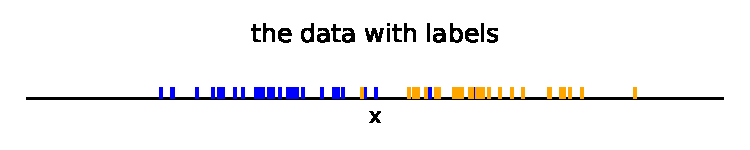
\includegraphics[width=0.8\textwidth]{img/latentexample_nofit_labels}
	\notesonly{\captionof{figure}{The labeling of points according to the group which we do not have.}}
\end{center}

We don't have any labels for the data and no access to the hidden causes. However, we can model these causes using latent variables.

\end{frame}

\begin{frame}{Assignment variables as latent variables}

A simple way to understand what latent variables represent is to view them as assignment variables to components that we need to estimate.

Example:\\

\begin{itemize} 
\item assignment variables: $\vec{m}^{(\alpha)} =  \big( m_1^{(\alpha)}, \dots, m_M^{(\alpha)} \big)^\top \in \left\{ 0, 1 \right\}^M$ \\
		\begin{align}
		m_q^{(\alpha)} &= 
		\begin{cases}
		1, & \text{if component } q \text{ has generated point}~\alpha\\
		0, & \text{otherwise}
		\end{cases}
		%\hspace{0.5cm}
		\;\text{with} \;
		 \sum_{q=1}^{M} m_q^{(\alpha)} = 1 
		\end{align}
\end{itemize}

\svspace{-7mm}

\notesonly{We have also see how Gaussian Mixture Models can model assignment variables using mixture components.}

\begin{center}
	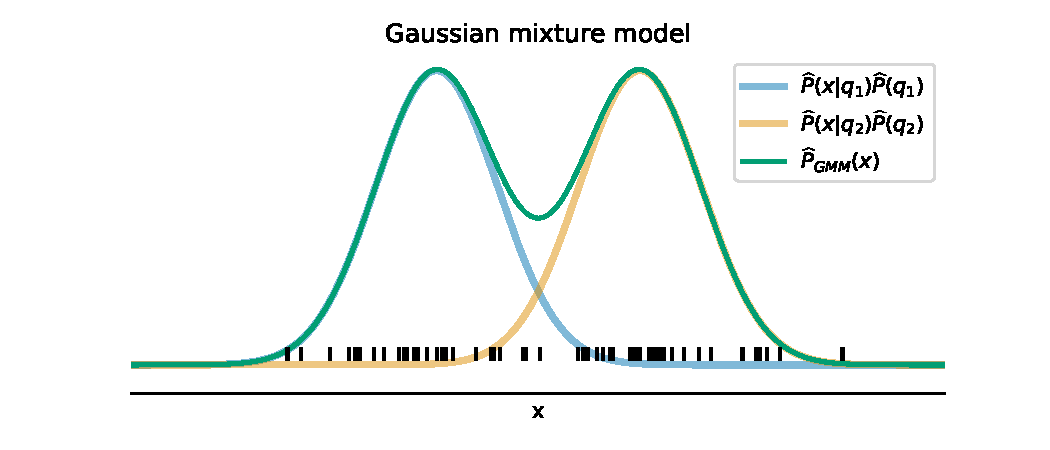
\includegraphics[width=0.7\textwidth]{img/latentexample_gmm}
	\notesonly{\captionof{figure}{A Gaussian Mixture Model as a latent variable model}}
\end{center}


\end{frame}

\begin{frame}{Latent variable models}

We view the data likelihood as a marginalization of the latent variables:

\begin{equation}
P \left( \left\{ \vec{x}^{(\alpha)} \right\} | \vec{w} \right) \stackrel{\text{iid}}{=} \prod_{\alpha=1}^{p} P \left( \vec{x}^{(\alpha)} | \vec{w} \right) = \prod_{\alpha=1}^{p}  \sum_{\vec{m}} P \left( \vec{x}^{(\alpha)}, \vec{m} | \vec{w} \right)
\end{equation}

The corresponding log-likelihood:

\begin{equation}
\ln P \left( \left\{ \vec{x}^{(\alpha)} \right\} | \vec{w} \right) = \sum_{\alpha=1}^{p}  \ln \left( \sum_{\vec{m}} P \left( \vec{x}^{(\alpha)}, \vec{m} | \vec{w} \right) \right)
\end{equation}

The sum in the logarithm prevents us from finding a closed-form solution.

\end{frame}

\begin{frame}{A chicken-and-egg problem}

The objective is to maximize the likelihood of the data. In addition to estimating the densities our latent variable models can also tune the assignment variables of the data points for the different components.
Modifying one will lead to a modification of the other.

\pause

\question{Where have we encountered this alternating behavior before?}

- K-means. But there we didn't dwell too much about any chicken-and-egg problem. Basing everything on Euclidean distance took care of this.


\end{frame}

\subsection{The EM algorithm}

\begin{frame}{\subsecname}

The EM algorithm is an iterative approximate solution to the chicken-and-egg problem.

\begin{block}{The chicken-and-egg problem}

We need to know who is assigned to which group in order to estimate the density of that group (i.e. identify which date influences a component $q$)\\
\textbf{But} we don't know the assignments.\\
To get the assignments we need the density of that group\ldots

\end{block}

\end{frame}

\begin{frame}

\slidesonly{
\begin{center}
	
\includegraphics[width=0.5\textwidth]{img/meme_cycle}
\end{center}
}

\end{frame}


%%%%%%%%%%%%%%%%%%%%%%%%%%%%%%%%%%%%%%%%%%%%%%%%%%%%%%
\begin{frame}{\subsecname}

\begin{figure}[!th]
\footnotesize
\removelatexerror
\small
\scalebox{.9}{   
	\begin{algorithm}[H]
		\DontPrintSemicolon
		initialization:
		Random initial densities (i.e. random initialization of density parameters)\\
		\vspace{1mm}
		\Repeat{change below tolerance}{
			\vspace{3mm}
			1. Use the densities to assign points to groups\\
			\vspace{3mm}
			2. Use the curent assignments to update the densities\\
			\vspace{3mm}
		}
		\caption{Outline of the EM alogrithm}
	\end{algorithm}
}
\end{figure}

\pause

\slidesonly{
\begin{center}
	
\includegraphics[width=0.3\textwidth]{img/meme_kmeans}
\end{center}
}

\notesonly{
If you find that the outline of the EM algorithm looks a lot like K-means, it's because K-means is a special case of EM.
}


\end{frame}

\begin{frame}{Does EM work?}

We now need reassurance that alternating between the steps improves both
\begin{itemize}
\item our assignments\\
AND\\
\item our densities
\end{itemize}

\end{frame}

